\documentclass{subfiles}
\begin{document}
Un filtro di convoluzione blur, o filtro di media, come suggerisce il nome, applica una sfocatura all'immagine.
Concettualmente, considerata un'immagine \(I\), si crea un kernel \(K\) con appositi valori e dimensioni, con lo scopo di creare una nuova immagine \(I'\),
secondo il seguente processo.

Partendo dal pixel più a sinistra e in alto dell'immagine \(I\), si sovrappone alla stessa \(K\).
Si procede effettuando un prodotto punto-punto tra gli elementi dell'immagine e il kernel, e se
\begin{wrapfigure}{r}{0.4\textwidth}
    \centering
    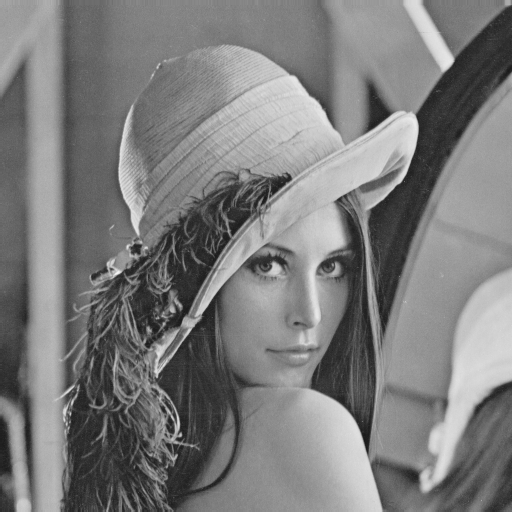
\includegraphics[scale = 0.3]{../Images/Lena/LenaGS.png}
    \caption{LenaGS}
    \label{fig:4.1}
\end{wrapfigure}
ne effettua una media.
Su una nuova immagine \(I'\) si aggiunge, nelle coordinate indicate dall'elemento centrale del kernel,
un pixel il cui colore è determinato dalla media precedentemente calcolata.
Si ripete il processo per tutta l'immagine, spostando \(K\) secondo una logica raster.

Per comprendere l'effettivo funzionamento del filtro, si supponga di dover applicare a \emph{Figura \ref{fig:4.1}} una sfocatura.
Come anticipato, la sfocatura dell'immagine è dipendete dalle dimensioni e dai valori del kernel.
Dunque al fine di comprendere tale differenza siano considerate \emph{Figura \ref{fig:4.2}}, ottenuta tramite convoluzione con un kernel 3 x 3 i cui pesi sono tanto maggiori,
tanto più vicini al centro; e \emph{Figura \ref{fig:4.3}} (mostrata nella sezione a seguire) ottenuta per convoluzione con un kernel 21 x 21, i cui pesi sono tutti unitari.

Partendo col considerare \emph{Figura \ref{fig:4.2}}, che come detto è ottenuta per convoluzione con il kernel 3 x 3 prima citato,
questa risulta pressoché immutata, cosa che invece non accade in \emph{Figura \ref{fig:4.3}} utilizzato il kernel 21 x 21.
\begin{wrapfigure}{l}{0.425\textwidth}
    \centering
    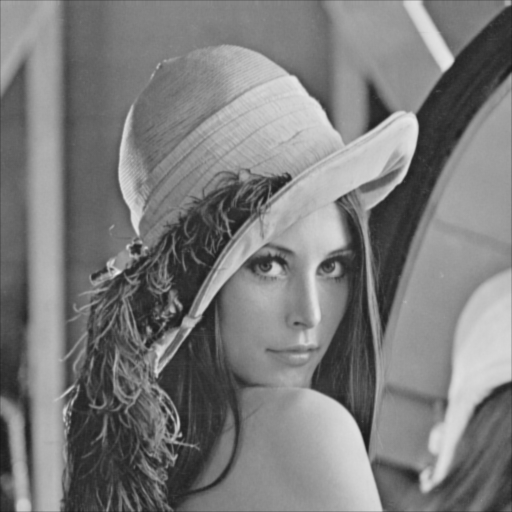
\includegraphics[scale = 0.325]{../Images/Lena/MeanConvolutionLena.png}
    \caption{Convoluzione di \emph{Figura \ref{fig:4.1}}, versione kernel 3 x 3.}
    \label{fig:4.2}
\end{wrapfigure}
La sfocatura è così minima da risultare impercettibile, sebbene se osservate da molto vicino risulta presente.

Sia ora considerato il seguente codice MATLAB.
\begin{center}
    \begin{lstlisting}[language = MATLAB]
        % caricamento dell'immagine Lena
        ker = [0 4 0; 4 8 4; 0 4 0]/24;
        convLena = conv2(single(Lena), ker, `same');
        figure; imshow(uint8(convLena), [0, 255]);
    \end{lstlisting}
\end{center}
Questi è utilizzato per ottenere \emph{Figura \ref{fig:4.2}}. Passando alla sua analisi, l'istruzione \lstinline[language = MATLAB]{ker = [...]/24;}
dichiara \emph{ker} come una matrice 3 x 3, i cui valori sono normalizzati evitando così perdita di informazioni;
l'istruzione \lstinline[language = MATLAB]{conv2(single(Lena), ker, `same')} effettua la convoluzione secondo quanto detto, tra l'immagine e \emph{ker}:
il parametro `same' è utilizzato per indicare la convoluzione deve lasciare il bordo immutato, il perché sarà chiaro dopo aver letto la sezione a seguire.

\begin{Note*}
    il cast a single, corrispettivo del \lstinline[language = C]{float} in C, è necessario per via implementazione della funzione \lstinline[language = MATLAB]{conv2};
    quello a uint8, corrispettivo dell'\lstinline[language = C]{inc} in C, non è strettamente necessario.
\end{Note*}
\clearpage

\subsubsection{Problema ai bordi}
Il filtro di media soffre di un grave problema, il cosiddetto \emph{problema ai bordi}.
Sebbene ottenuta con il filtro di blur, \emph{Figura \ref{fig:4.2}} sembra non presentare tale problema:
si osservi però che il
\begin{wrapfigure}[13]{r}{0.425\textwidth}
    \centering
    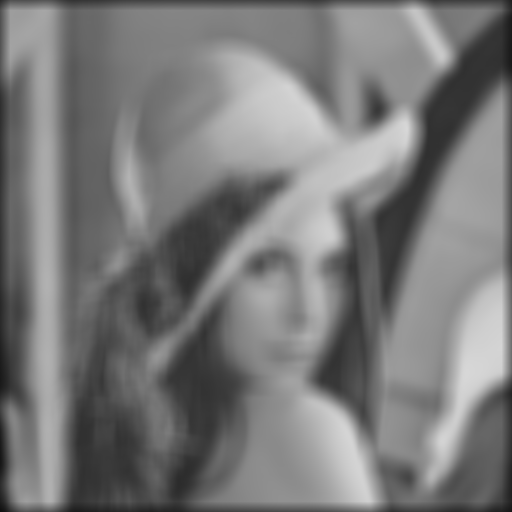
\includegraphics[scale = 0.325]{../Images/Lena/MeanConvolutionLena_21x21.png}
    \caption{Convoluzione di \emph{Figura \ref{fig:4.1}}, versione kernel 21x21.}
    \label{fig:4.3}
\end{wrapfigure}
kernel utilizzato è di dimensioni minime, quindi un problema di un pixel di spessore risulta impercettibile.

Per comprendere l'effettiva presenza di tale problema, che tra l'altro non ammette soluzione concreta, si consideri \emph{Figura \ref{fig:4.3}}.
Questa, ottenuta ottenuta eseguendo il seguente codice MATLAB, presenta evidenti differenze rispetto \emph{Figura \ref{fig:4.2}}.
\begin{center}
    \begin{lstlisting}[language = MATLAB]
        % si aggiunge l'immagine trascinandola in MATLAB
        ker = ones(21)/441;
        convLena = conv2(double(Lena), ker, `same');
        figure; imshow(uint8(convLena), [0, 255]);
    \end{lstlisting}
\end{center}
Tralasciando il grado di sfocatura che ovviamente risulta essere maggiore, è evidente la presenza di un bordo tendete al nero.

Si è detto che il filtro blur, come un pò tutti i filtri convolutivi, è soggetto al problema ai bordi.
Ciò non è pero sorprendente: proprio per la definizione stessa di filtro di convoluzione, che come ormai noto considera il pixel identificato dall'elemento centrale del kernel,
la convoluzione dei pixel al bordo non è possibile, dando così vita al problema.

Come anticipato il problema ai bordi non ammette una soluzione concreta, esistono comunque tecniche che permettono di ``alleggerirlo''.
Considerandone alcune, queste sono le seguenti
\begin{itemize}
    \item L'immagine viene viene estesa in ogni direzione con un bordo di pixel neri. Tale bordo deve essere sufficientemente largo da permettere di effettuare la convoluzione,
          a seguito della quale l'immagine è ritagliata per ottenere le dimensioni dell'immagine di partenza.
          \`E quel che si è fatto con \emph{Figura \ref{fig:4.3}} utilizzando il parametro `same'.

    \item Si considera la convoluzione esatta: si procede con la convoluzione e si ritaglia l'immagine limitandosi a quei pixel su cui effettivamente è avvenuta la convoluzione,
          pertanto si riducono le dimensioni dell'immagine. Sebbene si possa considerare la scelta più corretta,
          si tenga a mente che all'aumentare delle dimensioni del kernel aumenta il numero di pixel di bordo rimossi.

    \item L'immagine è resa periodica: si ripete l'immagine in ogni direzione e si procede con la convoluzione.
          Ottima da un punto di vista teorico matematico, risulta pessima in quanto presenta possibili punti di discontinuità di colore,
          che renderebbero falsata l'immagine finale.

    \item Si rende l'immagine periodica secondo uno schema a mosaico: similarmente a prima l'immagine è ripetuta in tutte le direzioni,
          con la differenza che l'immagine viene specchiata opportunamente, procedendo successivamente con la convoluzione.
\end{itemize}
\end{document}